\documentclass{article}

\usepackage{listings}
\usepackage{graphicx}
\usepackage{cite}
\usepackage{url}
\usepackage{listings}
\usepackage[margin=0.5in]{geometry}

\title{BRS Readout Description}
\author{M.P.Ross}
\begin{document}
\maketitle
\section{Introduction}
This document describes the ``BRSReadout'' software which was developed by the E{\"o}t-Wash group as the readout software of the Beam Rotation Sensor (BRS). The BRS's angular readout is achieved using a multi-slit autocollimator refined from the device described in \cite{autoCol}. The goal of the software is to turn line camera images into an number of angular readout channels, which are set to the accompanying TwinCAT code, while also giving the user an interface to view the camera images, plot the angular data, record data to disk, and monitor performance. The source for BRSReadout software can be found here: \url{https://github.com/mpross/BRSReadout} or \url{slowcontrols/trunk/BRS2 C#/BRSReadout/}. The accompanying TwinCAT code can be found at \url{slowcontrols/trunk/TwinCAT3/BRS/} with a version for each BRS deployed at the observatories.

\section{Overview}
The code is split between a number of simultaneous threads to allow for increased functionality while maintaining performance. The core of the software is the Form1.cs class which analyzes the images as described in the Image Analysis section, calculates the various signals and status bits, and handles all of the data communication with other threads and the accompanying TwinCAT code. The graphing (Form2.cs), frame capturing (Camera.cs), and data writing (DataWriting.cs) are all handled in their own threads to allow the various subroutines to run at different rates while also decoupling the performance of the threads.

Upon initialization, the main loop starts the other threads, reads a collection of settings from the configuration files, and triggers the camera to begin continuous acquisition. After which is waits for a frame to come into the queue before running the frame through the analysis, calculating signals, then sending the signals to the other threads and the TwinCAT code. It then waits for another frame and repeats until the software is closed. It should be noted that the analysis is highly CPU intensive and requires a dedicated core to achieve maximal rate while avoiding interrupts from other processes. This is achieved by utilizing the CPU Affinity setting in Windows which is set using a the AffinitySet.bat script on startup. 
\begin{center}
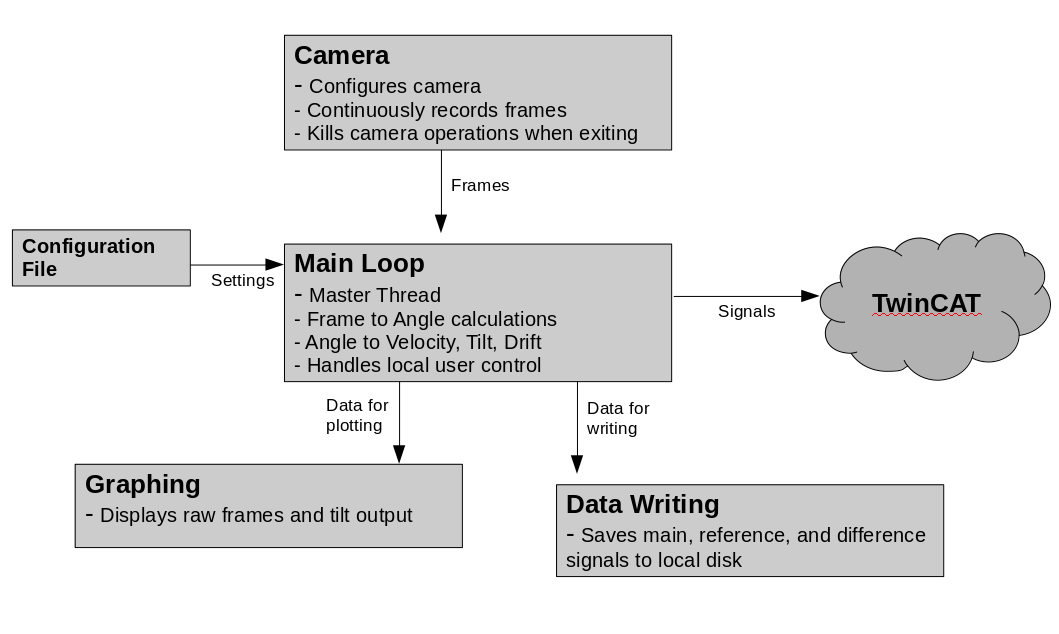
\includegraphics[width=0.75\textwidth]{BRSReadoutFlow.png}\\
\end{center}

\section{Image Analysis}
The multi-slit autocollimator shines light from a fiber coupled LED through a mask consisting of 38 slits which is then set through a beam splitter. The reflected beam is imaged onto a CCD line camera while the transmitted beam reflects off of a mirror that is attached to the beam before also being imaged on the CCD. This forms two nearly identical patterns, the reference and main patterns which respectively correspond to the reflected and transmitted path of the beam splitter. The major differences between the patterns is the height of the peaks which is due to the main pattern passing through the beam splitter twice and the spatial separation of the two patterns which is due to a static angle between the main mirror and the optical path. Introducing this static angle also reflects away the secondary reflections out of the imaging plane of the CCD.\\

\begin{center}
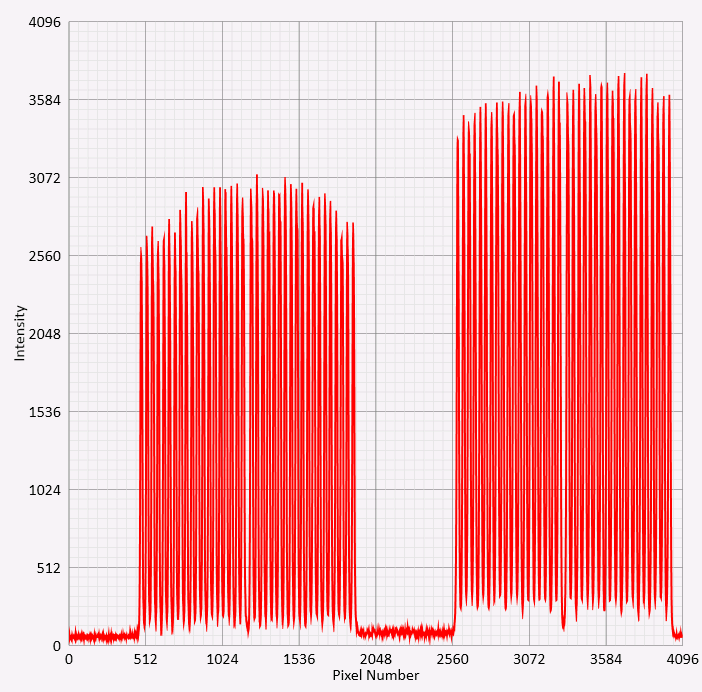
\includegraphics[width=0.5\textwidth]{BRSReadoutScreenPatterns.png}\\
\end{center}

As the angle between the beam and the housing change, the main pattern (shown above on the left) translates across the CCD while the reference pattern stays stationary. The program now needs to take these images and turn it a data stream of angular readings by measuring the distance between the patterns for each frame.

The frames are recorded by the camera as a 4096 element vector of 12 bit numbers representing the intensity of each CCD pixel. The control of the camera and initial frame handling is done in the Camera.cs class which pulls the frames from the camera using the Basler Pylon APIs, averages a small number of frames together to decrease downstream load, and puts them in a queue to be ready by the main loop. Additionally, for some of the BRSs the cameras were intentionally installed backwards. To account for this each frame is reversed before being sent on.\\

\textbf{Frame recording code (Camera.startFrameGrab)}:
\begin{lstlisting}{sharpc}
while (true)
{
	if (cameraType == "basler")
	{
	    PylonBuffer<Byte> buffer;
	    Pylon.WaitObjectWait(hWait, 100);

	    Pylon.StreamGrabberRetrieveResult(hGrabber, out grabResult);

	    bufferIndex = (int)grabResult.Context;

	    while (buffers.TryGetValue(grabResult.hBuffer, out buffer) != true) ;
	    Buffer.BlockCopy(buffer.Array, 0, data, 0, buffer.Array.Length);

	    if (frameReverse)
	    {
		Array.Reverse(data);
	    }
	    frameAveraging(data);
	    Pylon.StreamGrabberQueueBuffer(hGrabber, grabResult.hBuffer, bufferIndex);
	}
}
\end{lstlisting}

Once a frame is placed in the queue the main loop (Form1.cs) retrieves it and under goes a series of steps to extract the position of each pattern. The first step of this process is to split the frame in half and designating one side at the reference pattern and the other as the main pattern. This splitting is done at a static location that can be set by changing the "splitPixel" parameter in the configuration file and is normally set to be as close to the reference pattern as possible. This is to give the main pattern, which will be moving during operation, the most room possible. From here on the patterns are treated as separate and undergo identical analyses to yield two channels, the main channel and the reference channel, which correspond to the location of the respective patterns.

To give the algorithm a frame to compare with, the first frame that comes into the algorithm is saved and treated as a standard against which all future frames will be compared. Since this frame is captured on the given instrument, it will contain similar nuance features as future frames and thus be  a better standard than any theoretical pattern. This frame is stored and used until either the software is restarted or the "Recapture Frame" button is pressing. This recapture function is only necessary if the first frame is corrupted due to a bad camera frame or if either pattern is out of range.

Once another frame comes in, the algorithm must extract the current position of the two patterns with respective to their position in the first frame. This is done by combining two methods: a course threshold based edge finder and a fine cross correlation based center calculation. The edge finder finds the first pixel that has an intensity greater than the threshold that is set by the "threshold" parameter in the configuration file. A number set by the "pixelMargin" parameter is subtracted from this pixel number to ensure that the entire pattern is used in the cross correlation step. This is then saved as the "startIndex" and provides a measure of the patterns location to within a pixel. \\

\textbf{Edge finding code (Form1.Pattern)}:
\begin{lstlisting}{sharpc}                    
for (int j = splitPixel; j < frame.Length; j++)
{
	if (frame[j] > threshold)
	{
    		startIndexRight = j - pixelMargin;
		break;
	}
	if (j == frame.Length-1)
	{
		startIndexRight = 0;
	}
}
\end{lstlisting}

To get sub-pixel resolution of the position, we take the cross correlation of the section of the current frame from the start index to the start index plus the pattern length (which is set by the "patternLength" parameter) and the corresponding section in the first frame. This gives us a oscillating pattern with a central peak that is displaced from zero by the distance between the patterns. A gaussian is then fit to a number of points around this central peak. The mean value of this gaussian then corresponds to the sub-pixel displacement of the pattern and it's respective first frame pattern. This is then added to the start index to yield an accurate measure of the patterns location.\\

\textbf{Cross correlation code (Form1.Pattern)}:
\begin{lstlisting}{sharpc}    
for (int k = -halflength; k <= halflength; k++)
{
	sum = 0;
	for (int m = 0; m < length; m++)
	{
		if ((m + startIndexRight + k) > 0 && (m + startIndexRightRef) > 0)
		{
			if ((m + startIndexRight + k) < frame.Length 
				&& (m + startIndexRightRef) < refFrame.Length)
			{
				sum += frame[m + startIndexRight + k] 
					* refFrame[m + startIndexRightRef];
			}
		}
	}
	crossCor[k + halflength] = sum;
}

//Sums x,x^2,x^3,x^4,ln(y),x ln(y),x^2 ln(y)
y = 0;
xy = 0;
xxy = 0;

for (int j = 0; j < fitLength; j++)
{
	y += Math.Log(crossCor[j + 1]);
	xy += j * Math.Log(crossCor[j + 1]);
	xxy += j * j * Math.Log(crossCor[j + 1]);
}
//Solves system of equations using Cramer's rule
D = N * (xSquar * xFourth - xCube * xCube) 
	- x * (x * xFourth - xCube * xSquar) + xSquar * (x * xCube - xSquar * xSquar);
//Da = y * (xSquar * xFourth - xCube * xCube) 
	- x * (xy * xFourth - xCube * xxy) + xSquar * (xy * xCube - xSquar * xxy);
Db = N * (xy * xFourth - xCube * xxy) 
	- y * (x * xFourth - xCube * xSquar) + xSquar * (x * xxy - xy * xSquar);
Dc = N * (xSquar * xxy - xy * xCube) 
	- x * (x * xxy - xy * xSquar) + y * (x * xCube - xSquar * xSquar);
//a = Da / D;
b = Db / D;
c = Dc / D;

mu = -b / (2 * c);

newdata[frameNo, 0] = mu + startIndexRight;
timestamps[frameNo] = data.TimeStamp(frameNo);

angleLastValue = mu + startIndexRight;

\end{lstlisting}

Once both patterns go through this procedure, the algorithm outputs two data streams: the raw reference pattern motion as a measure of the instruments readout noise and the difference between the two patterns which will be proportional to the tilt with decreased contribution of the readout noise due to the subtraction. These two channels are then sent on to the graphing thread, the data writing thread, and to the signal processing to be calibrated, conditioned, and split into the various output channels.

A demonstration of this analysis can be seen in the accompanying BRSReadoutDescription.m Matlab script.

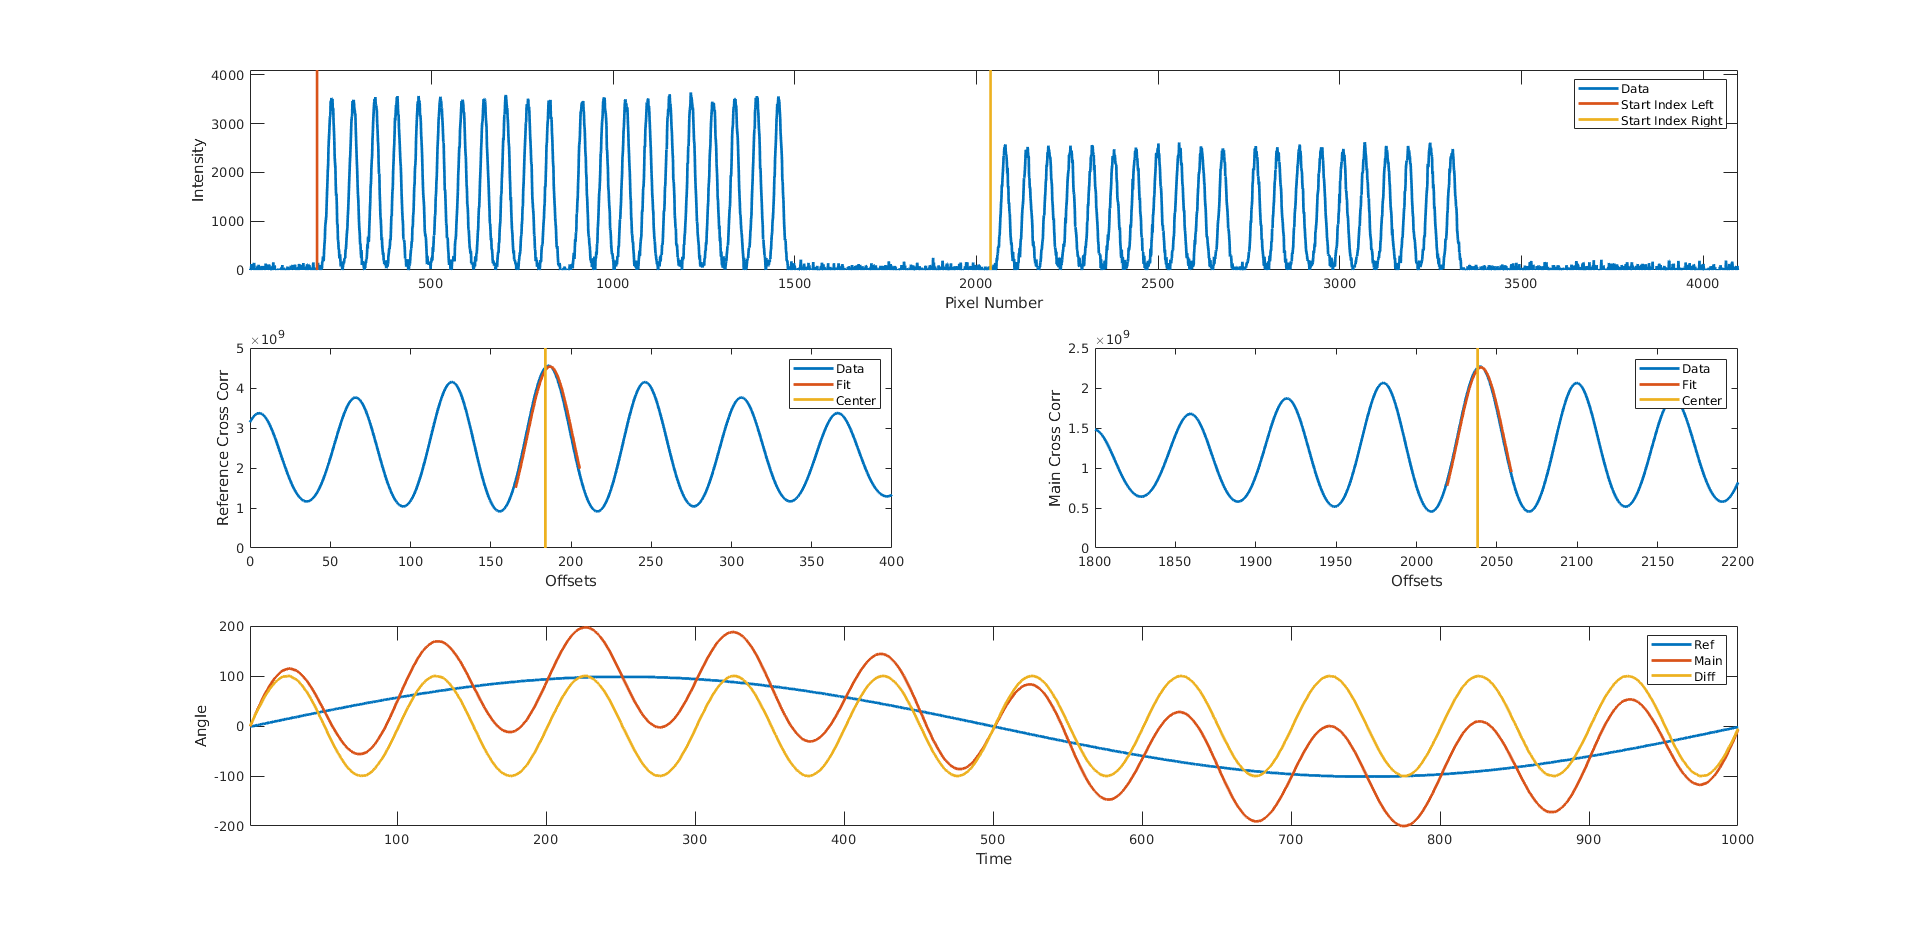
\includegraphics[width=\textwidth]{Demonstration.png}\\

\section{Signal Processing}

Under normal conditions the raw angle (difference) signal can take on a significant range of values. Since these signals will be sent to the seismic front ends using DACs, using only the raw signal would lead to significant bit noise. To circumvent this the angle signal is split into two: a drift channel which is raw signal with a gain which matches the dynamic range of the autocollimator to the range of the DACs and a tilt signal which passed through a roughly 1 mHz high pass filter before being calibrated to 1 nrad per DAC count. The tilt channel is then a low noise signal that can be sent on to the control systems while the drift channels allow for a diagnostic monitor that ensures that the instrument is in range while being used. To allow the device to output a drift channel while the main pattern is off the edge of the CCD, the drift channel can be rescaled and recentered by triggering the "Drift override" state. \textbf{This compromises the fidelity of the tilt channel and should only be used during diagnostics.}

In addition, the instrument has two capacitor plates that are used to damp the amplitude of the beam. This requires the velocity of the angular motion around the resonant frequency of the beam which is calculated by band passing the tilt signal around the resonance (3-8 mHz) and then taking the difference. This is then square rooted to account for the fact that the force between capacitor plates goes as the voltage squared and  then limited to be within the DACs range.

The tilt, drift, velocity, and reference channels are then sent out to the accompanying TwinCAT code in addition to a selection of status bits. These give the status of whether the Readout code is running, whether the camera is getting enough light, and whether the communication with the camera is functioning. Once these signals are sent the main loop cycles through for another frame until the software is shutdown.
\\

\textbf{Signal processing code (Form1.dataSend)}:
\begin{lstlisting}{sharpc}   
angle = data[0];
refAng = refGain * (data[1] - refZeroValue);
//Has a DC subtraction to help filters. Should be about the center of the signal.
if (firstValueCounter < 40)
{
	firstValueCounter++;
	zeroValue = data[0];
	refZeroValue = data[1];
}
xHighPass[0] = angle - zeroValue;
xBandLowPass[0] = angle - zeroValue;

//Drift signal calculation, just scaled signal
if (dampOverride)
{
	drift = driftOverGain * (angle - driftOverOffset);
}
else
{
	drift = driftGain * (angle - driftOffset);
}
//Drift rail logic
if (Math.Abs(drift) >= 32760)
{
	drift = Math.Sign(drift) * 32760;

}

//Tilt signal calculations, high pass at 10^-3 Hz then scaling.
yHighPass[0] = highCoeff[3] * yHighPass[1] + highCoeff[4] * yHighPass[2] 
		+ highCoeff[0] * xHighPass[0] + highCoeff[1] * xHighPass[1] 
		+ highCoeff[2] * xHighPass[2];
tilt = angleGain * yHighPass[0];

//Capacitor signal calculations, low passed at Hz then high passed 
	at Hz then differentiated and scaled
yBandLowPass[0] = bandLowCoeff[3] * yBandLowPass[1] + bandLowCoeff[4] * yBandLowPass[2] 
		+ bandLowCoeff[0] * xBandLowPass[0] + bandLowCoeff[1] * xBandLowPass[1]
		+ bandLowCoeff[2] * xBandLowPass[2];
xBandHighPass[0] = yBandLowPass[0];
yBandHighPass[0] = bandHighCoeff[3] * yBandHighPass[1] + bandHighCoeff[4] * yBandHighPass[2] 
		+ bandHighCoeff[0] * xBandHighPass[0] + bandHighCoeff[1] * xBandHighPass[1] 
		+ bandHighCoeff[2] * xBandHighPass[2];
velocity = velGain* Math.Round((double)200 / bufferSize) * 
			(yBandHighPass[0] - yBandHighPass[1]);


if (velocity > 0)
{
	velocity = Math.Sqrt(velocity);
}
else
{
	velocity = -Math.Sqrt(-velocity);
}

if (Math.Abs(velocity) >= 30760)
{
	velocity = Math.Sign(velocity) * 30760;
}
if (twinCatBool)
{
	ds = new AdsStream(28);
	BinaryWriter bw = new BinaryWriter(ds);
	//Tilt signal. TwinCAT variable tilt at MW0.
	bw.Write((int)tilt);
	//Drift signal. TwinCAT variable drift at MW1
	bw.Write((int)drift);
	//Velocity signal. TwinCAT variable cap at MW2
	bw.Write((int)velocity);
	voltagewrite = velocity / 3276;
	//Reference signal. TwinCAT variable ref at MW3
	bw.Write((int)refAng);
	//C# pulse. Sets TwinCAT variable cPulse=1 at MW4
	bw.Write((int)1);
	//Light source status bit at MW5
	bw.Write((int)lightSourceStatus);
	//Camera status bit at MW6
	bw.Write((int)cameraStatus);
	tcAds.Write(0x4020, 0, ds);
}
\end{lstlisting}

\section{User Interface}

The user interface is design to mainly to allow a local user to monitor the status of the software and device while also allow some limited user controls. It is split between two separate windows, "BRS Readout" and "BRS Graph", corresponding to the Form1.cs and Form2.cs classes. These run in independent threads to decouple the performance of the graphing from the main loop while also utilizing multiple cores.

"BRS Readout" is the main window which will be open whenever the software is running and holds all of the user controls. It displays four statistics at the top of the panel: time since the code was run in seconds, the length of the camera queue and the graphing queue, and the voltage being written to the capacitor plates. These are used as diagnostics to ensure that the code is running as expected. The panel also has five buttons which give the user the ability to record the data to the local disk, clear the angle graph, recapture the first frame, open the graphing window, and to turn on the damping override. The ability to record to disk does not affect the output data streams but is intended to allow the BRS to collect data without communicating with the LIGO systems. The frame recapture function can be used if the first frame captured by the camera is corrupted while the damping override will allow the BRS to damp the beam motion even if the main pattern is slightly off the CCD. \textbf{This compromises the fidelity of the tilt channel and should only be used during diagnostics.}

\begin{center}
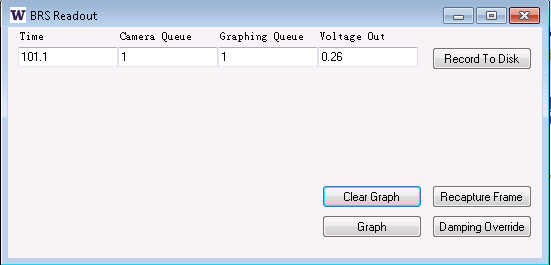
\includegraphics[width=0.5\textwidth]{BRSReadoutScreen.png}\\
\end{center}

The "BRS Graph" window hold two panes which show plots of the current frame on the left and a time series of the angular output on the right. This allows the user to get a image of the patterns 

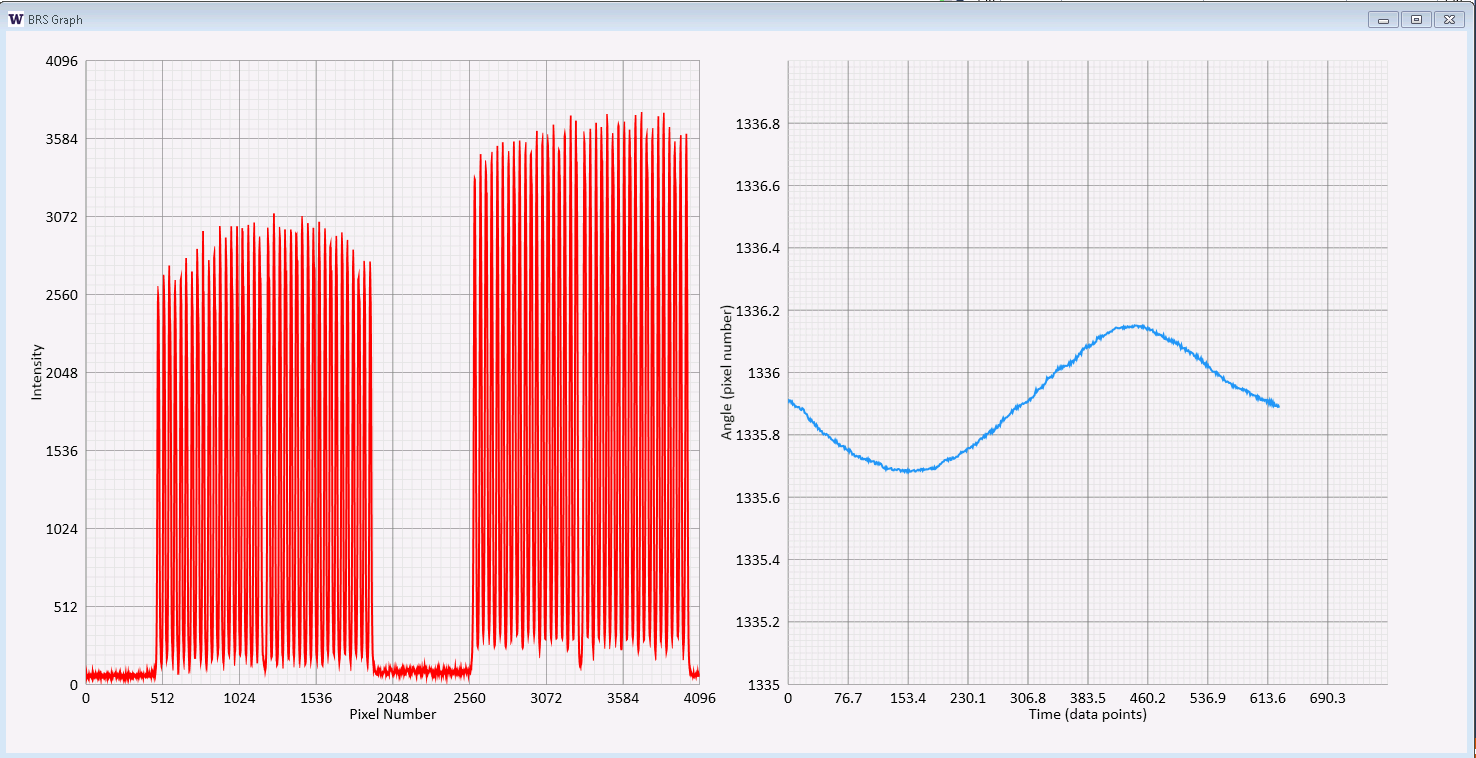
\includegraphics[width=\textwidth]{BRSReadoutScreenGraph.png}
\section{Configuration File}

General settings
\begin{itemize}
\item location - Device location name. Example: LHO End-X
\item twinCat - Boolean controlling use of TwinCAT software. Default: true
\end{itemize}
Camera settings
\begin{itemize}
\item camera - Camera type. Default: basler
\item cameraBitDepth - Camera bit depth. Default: 12
\item cameraExposureTime - Camera exposure time. Default: 500
\item cameraWidth - Camera pixel number. Default: 4096
\item ipAddress - IP Address of camera. Only needed for cameras that are routed through switch.
\item frameAverageNum - Number of frames to average within Camera class. Default: 4
\item frameReverse - Frame flip boolean. Only true for devices with camera installed backwards.
\end{itemize}
Graphing settings
\begin{itemize}
\item graphingFrameNumber - Number of frames to wait until graph is updated. Default: 5
\item bufferSize - Number on frames in buffer. Default: 20
\item numberOfGraphPoints - Number of points to graph. Default: 1000
Email settings
\item emailList - List of emails to send crash reports to separated by ",".
\end{itemize}
Filter settings
\begin{itemize}
\item angleLowPass - Cutoff frequency for tilt low pass in Hz. Default: 0.1
\item angleHighPass - Cutoff frequency for tilt high pass in Hz. Default: 0.0005
\item velocityLowPass - Cutoff frequency for velocity low pass in Hz. Default: 0.02
\item velocityHighPass - Cutoff frequency for velocity high pass in Hz. Default: 0.002
\end{itemize}
Fitting settings
\begin{itemize}
\item threshold - Edge finder threshold. Default: 1200
\item splitPixel - Pixel on which frame is split between patterns. Default: 1800
\item pixelMargin - Margin to shift back by in edge finding to ensure entire pattern is captured. Default: 40
\item patternLength - Pattern length. Default: 1500
\end{itemize}
Gain settings
\begin{itemize}
\item refGain - Reference channel gain. Default: 3499.8
\item angleGain - Angle channel gain. Default: 3645
\item velGain - Velocity channel gain. Default: -5000000000
\item driftGain - Drift channel gain. Default: 60
\item driftOffset - Drift channel offset. Default: 2146
\item driftOverGain - Drift channel gain during override. Default: 30
\item driftOverOffset - Drift channel offset during override. Default: 2646
\end{itemize}

\section{Troubleshooting}
\section{Previous Versions}
Although this document was written specifically about the "BRSReadout" software, previous version such as the "FringeAutocollimator" software follow an almost identical image analysis and have similar GUI components.
\bibliographystyle{plain}
\bibliography{ReadoutDescription}{}
\end{document}